The term \textit{Motion Primitives} has its roots in neurobiology and motor control, where researchers
explain the execution of complex motion of biological systems and their ability to adapt to different types of motion effortlessly.
The Dynamic Motion Primitives formulation is one among the many that use the popular approach in \textit{Robot Learning} called Learning from Demonstrations, which uses the demonstrations given by a 
human in some form (teleoperation, kinesthetic control etc\dots) and learn from it to scale to different tasks for robot to perform.
% ! TODO: Add more details and cite the LFD article. 
In this respect, DMPs attempt to answer the question:

\begin{quote}
    \centering
    \textit{How artificial systems can execute
complex movements in a versatile and creative manner?\cite{saveriano2021dynamic}}
\end{quote}

Thus, Dynamic Motion Primitives (DMPs) can be seen as rigorous mathematical formulation of motion primitives as stable nonlinear dyanmical systems.

\section{Dynamics of DMPs}

At the heart of DMP lies a spring mass damper system.

\begin{equation}
    \tau \ddot{y} = \alpha \left( -\beta \left( y - y_g \right) - \dot{y} \right)
    \label{eq:dmp_equation}
\end{equation}

where $\alpha$ and $\beta$ are the constants of the spring mass damper system, $y_g$ is the goal state of the system. To avoid overshooting or slow convergence of the system to the goal state,
the system is set to be critically damped. Thus in the DMP notation, $\beta=\alpha/4$. This determine the value of $\beta$ for a given value of $\alpha$.

The infulence of $\alpha$ on the DMP system can be seen in Fig. \ref{fig:dmp_alpha_influence}.

% ! TODO: add figure for the dependance of alpha on the system. MAYBE USE DESMOS FOR THE SAME.???
\begin{figure}[h]
    \centering
    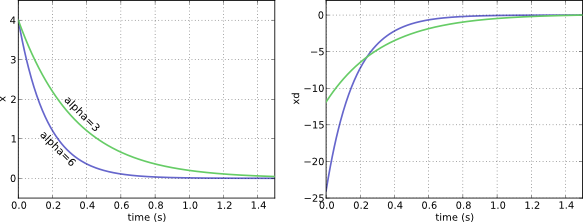
\includegraphics[width=0.8\textwidth]{dmp_alpha.png}
    \caption{DMP system with different values of $\alpha$} % edit with influence.
    \label{fig:dmp_alpha_influence}
\end{figure}

This representation has properties such as convergence to goal state and robutnesss to external perburtation but
can only represent very simple movements. To solve this we add a time dependaant forcing term to the spring mass damper system. The spring damper system
along with the forcing term is called as \textit{transformation system}.

After adding forcing term to our sping damp system, the we can no longer gurantee the convergence property and the tranformation system is no longer time independant.
To solve the later we let $f$ be a function of a phase variable $x$ representing the phase of the movement. A first order dynamical system
was used to model the phase variable in \cite{Ijspeert2002}, coining the term \textit{canonical system}.

Thus the complete Dynamic Motion Primitives system is given by:

\begin{subequations}\label{eq:dmpSystem}
    
    \begin{align}
        \tau \dot{z}& = \alpha_z (\beta_z \left( z - z_g \right) - \dot{z}) + f(x)\label{Tsystem}\\
        \tau \dot{y}& = z \\
        \tau \dot{x}& = \alpha_x x\label{cSystem}
    \end{align}
\end{subequations}

\begin{figure}[h]
    \centering
    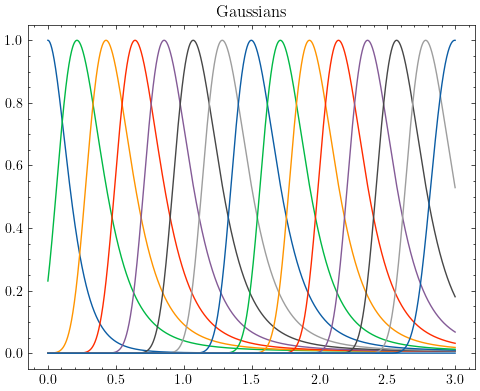
\includegraphics[width=0.7\textwidth]{gaussians}
    \caption{Gaussian Activations in Time}
    \label{fig:gaussians}
\end{figure}
where, $z$ is the state of the system, $x$ is the canonical variable, $f(x)$ is the non linear forcing term. And as described above, parameters
$\alpha_z$ define the charaterics of the DMP system, and with $\tau > 0 $, $\beta_z =  \alpha_z/4$ and $\alpha_x >0$ the convergence to 
goal state is guaranteed.

The term $f(x)$ is defined as the linear combination of $N$ nonlinear Radial Basis Functions (RBF) which are also known as Gaussian basis functions.
This enables the DMP to follow any arbitrary smooth trajectory from initial point $y_0$ to final position $y_g$.

\begin{align}\label{eq:dmp_rbf}
    f(x) &= \ddfrac{\sum\limits_{i=1}^{N} w_i \Psi_i(x)}{\sum\limits_{i=1}^N \Psi_i(x)}  x\\
    \Psi_i(x) &= e^{-h_i(x-c_i)^2}
\end{align}
where $h_i$ are the centers of the RBF, and $c_i$ are the centers of the RBF for $i = 1,2, \dots , N$. The weights $w_i$ are found oout from the measured 
data so that the desired trajectory is achieved. Fig. \ref{fig:gaussians} shows the Gaussian activations in time.
We can define the venters and widths as


\begin{align}
    c_i &= e^{-\alpha_x \ddfrac{i-1}{N-1}}\\
    h_i &= \ddfrac{1}{(c_{i+1} - c_i)^2}
\end{align}
where $h_N = h_{N-1}$. The selection of the number of weights and hence the RBF's is decided based on the accuracy required.
But it is observed that a certain minimum number of RBF's is required to encode the trajectory any meaningful manner\cite{saveriano2021dynamic}.

% %% ^ Section header for Learning the demonstration.
\section{Learning from demonstration}
For a discrete motion, given a demostrated trajectory $y_d(t_j)$, where $t_j = 1, \dots , \mathcal{T}$ is the number of time steps, and 
its time derivatives $\dot{y}(t_j)$ and $\ddot{y}(t_j)$, we can invert equation \eqref{Tsystem} to approximate
the desired forcing term.

\begin{equation}
    f_d(t_j) = \tau^2 \ddot{y}(t_j) - \alpha_z (\beta_z (g - y_d(t_j))  - \tau \dot(y)_d(t_j)) \label{inverseDMP}
\end{equation}

Arranging the desired forcing term $f_d(t)$ and the unknoen weights $w_i$ into column vector such that, 
\[ 
 \bm{\mathcal{F}} = \left[ f_d(t_1), f_d(t_2), \dots , f_d(t_T) \right]^T 
    \text{and  }   \boldsymbol{w} = \left[ w_1, w_2, \dots , w_N \right]^T  
        \]
we obtain a linear system, 
\begin{equation}
    \boldsymbol{\Phi} \boldsymbol{w} = \bm{\mathcal{F}}
\end{equation}
where,

\begin{equation}
\boldsymbol{\Phi} = 
\begin{bmatrix}
 \ddfrac{\psi_1(x_1)}{\sum\limits_{i=1}^{N} \psi_i(x_1)}x_1 & \cdots & \ddfrac{\psi_N(x_1)}{\sum\limits_{i=1}^{N} \psi_i(x_1)}x_1 \\
\vdots & \ddots & \vdots \\
\ddfrac{\psi_1(x_\mathcal{T})}{\sum\limits_{i=1}^{N} \psi_i(x_\mathcal{T})}x_\mathcal{T} & \cdots & \ddfrac{\psi_N(x_\mathcal{T})}{\sum\limits_{i=1}^{N} \psi_i(x_\mathcal{T})}x_\mathcal{T} 
               
\end{bmatrix}
\end{equation}

\begin{figure}[h]
    \centering
    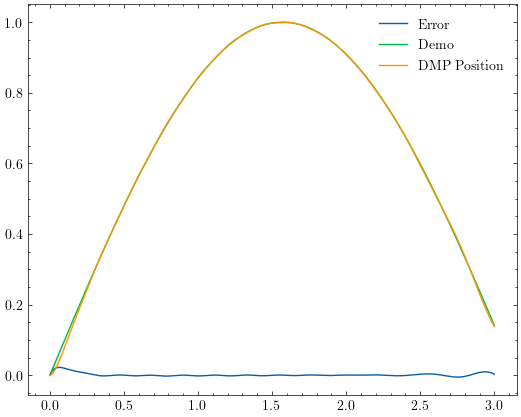
\includegraphics[width=0.8\textwidth]{1D_traj.png}
    \caption{A classical DMP is used to reproduce the trajectory of $x(t) = sin(t)$ for a total time of 3 seconds.} % replace the images with actual contect,
\end{figure}
This system can be solved by using various techniques such as the Least squares method, Locally Weighted Regression(LWR)\cite{LWR_paper} etc.
LWR is a popular approach to update the weights $w_i$ learned from the previous demonstration, using the error between the learned trajectory a
and desired trajectory by using a forgetting factor $\lambda$. In this project work, Least squares methods was used as it approximated test results accuratly.

\section{Temporal and Spatial Scalability of DMP}

The most important feature of DMP is that once trained on a certain training trajectory, it can replicate the trajectory
even when the goal and initial conditions are changed and follow it without requiring any additional training to train the weights\cite{Ijspeert2013}
\cite{ginesi2021overcoming}. This is called
as \textit{spatial scalability} of DMP.

\begin{figure}[h]
    \centering
    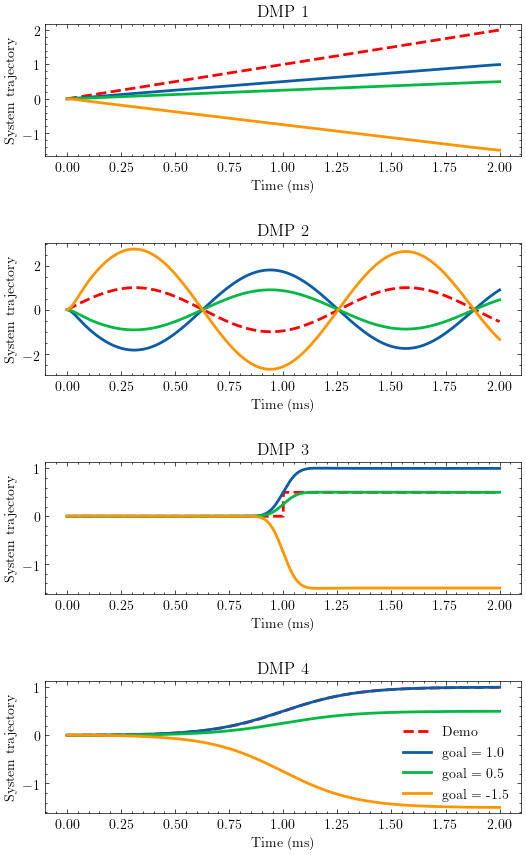
\includegraphics[height=0.7\textheight]{space_scale.png}
    \caption{The time constant $\tau$ is the parameter that controls the speed of the movement.}
\end{figure}
DMPs can also scale down or up a trajectory in the temporal direction by changing the time constant $\tau$, resulting in a shorter or longer trajectory time.
This is called \textit{temporal scalability} of DMP. The time constant $\tau$ is the parameter that controls the speed of the movement.
\begin{figure}[h]
    \centering
    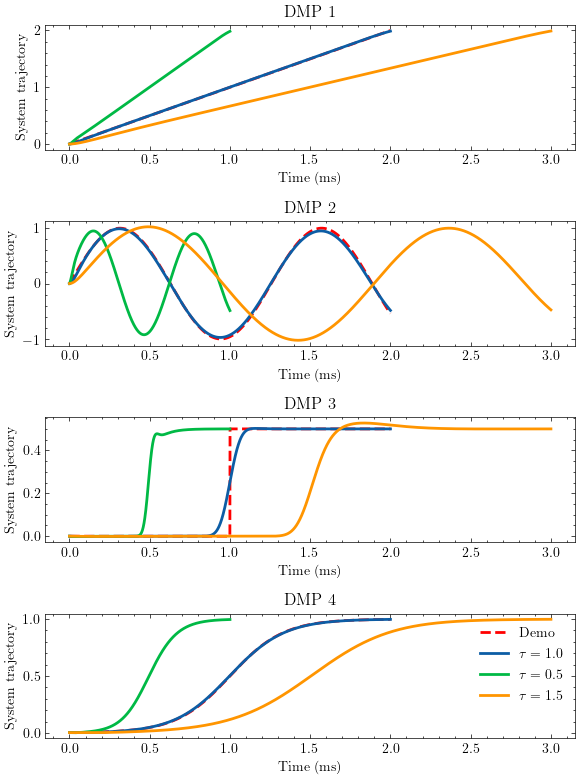
\includegraphics[height=0.7\textheight]{time_scale.png}
    \caption{The time constant $\tau$ is the parameter that controls the speed of the movement.}
\end{figure}

This property when mixed with joint DMP can provide a method for online adaptation of desired trajectory in robotic manipulators and other robotic systems.

This framework of DMP is called Discrete DMP. One of its main disadvantages is that it cannot encode the orientation of the trajectory into the system.
As such a new set of equations are transofrmaiton systems are created to handle this issues.